% Search for all the places that say "PUT SOMETHING HERE".

\documentclass[11pt]{article}
\usepackage{amsmath,textcomp,amssymb,geometry,graphicx,enumerate}
\graphicspath{ {images/} }

\title{CS189--FALL 2015 --- Homework 1 Write up}
\author{ZUBO GU, SID 25500921, gu.zubo@berkeley.edu, Kaggle id: ZUBO}
\markboth{}{}
\pagestyle{myheadings}
\date{}

\usepackage[procnames]{listings}
\usepackage{color}
\definecolor{keywords}{RGB}{255,0,90}
\definecolor{comments}{RGB}{0,0,113}
\definecolor{red}{RGB}{160,0,0}
\definecolor{green}{RGB}{0,150,0}
 
\lstset{language=Python, 
        basicstyle=\ttfamily\small, 
        keywordstyle=\color{keywords},
        commentstyle=\color{comments},
        stringstyle=\color{red},
        showstringspaces=false,
        identifierstyle=\color{green},
        procnamekeys={def,class}}

\textheight=9in
\textwidth=6.5in
\topmargin=-.75in
\oddsidemargin=0.25in
\evensidemargin=0.25in

\begin{document}
\maketitle

\section*{Problem 1. solution}

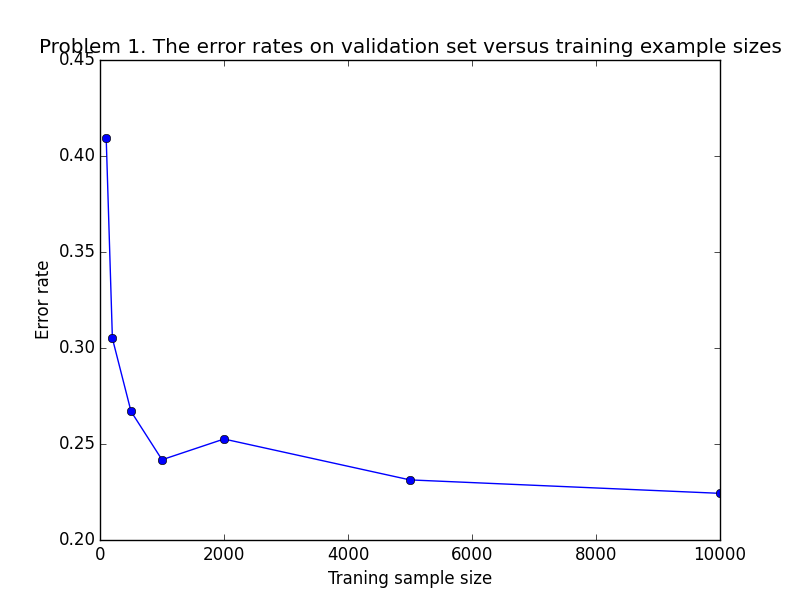
\includegraphics[scale=0.5]{figure1}

\newpage
\section*{Problem 2. solution}
From looking at the confusion matrix, I saw that(3, 8), (5, 8), (5, 3), (7, 9), (9, 4), (9, 8) are mostly miss predicted pairs.

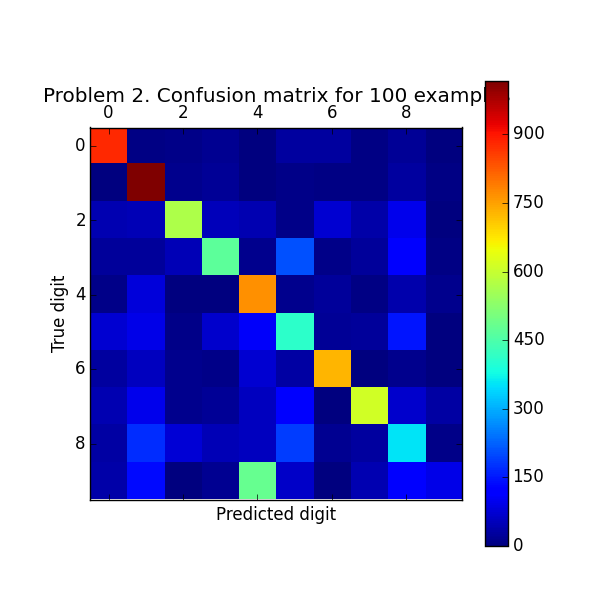
\includegraphics[scale=0.6]{figure2}
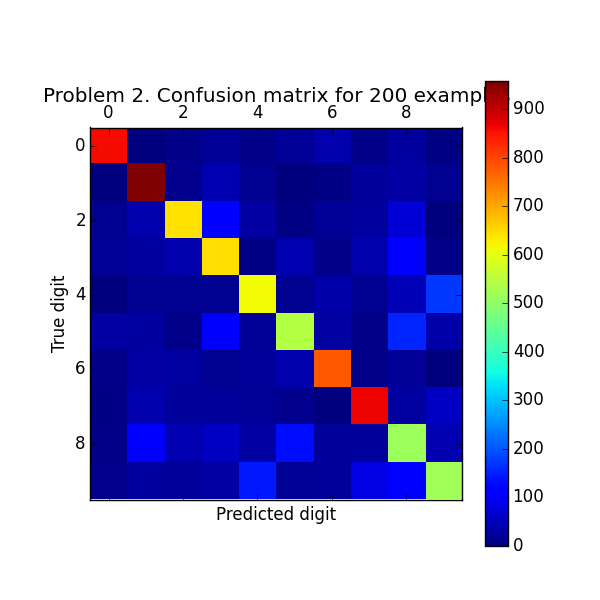
\includegraphics[scale=0.6]{figure3}

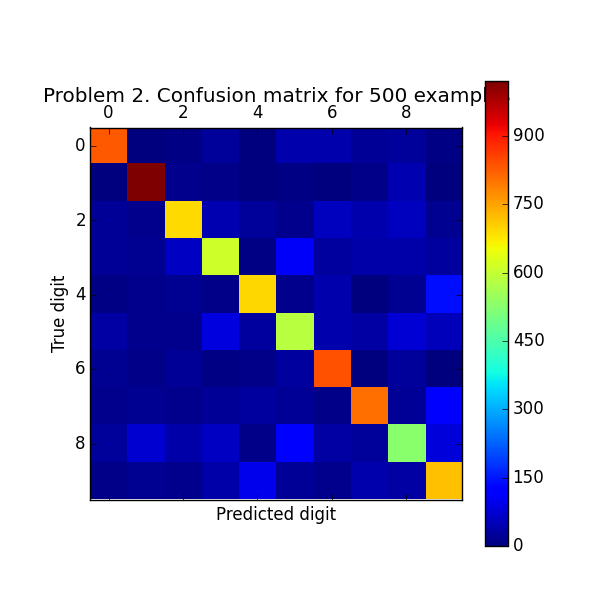
\includegraphics[scale=0.6]{figure4}
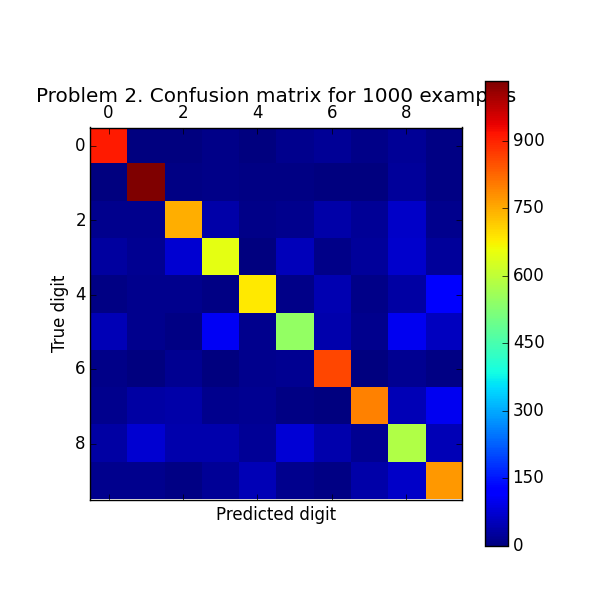
\includegraphics[scale=0.6]{figure5}

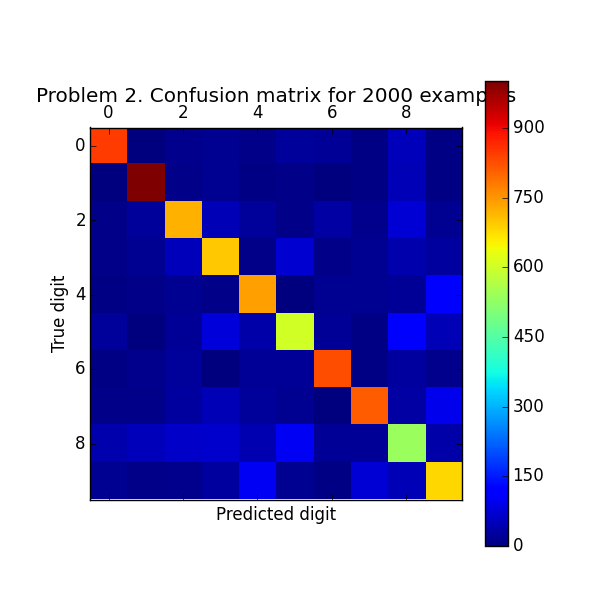
\includegraphics[scale=0.6]{figure6}
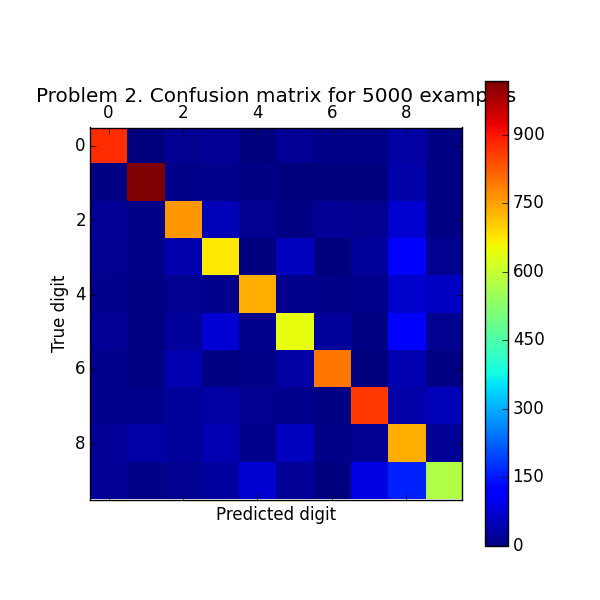
\includegraphics[scale=0.6]{figure7}

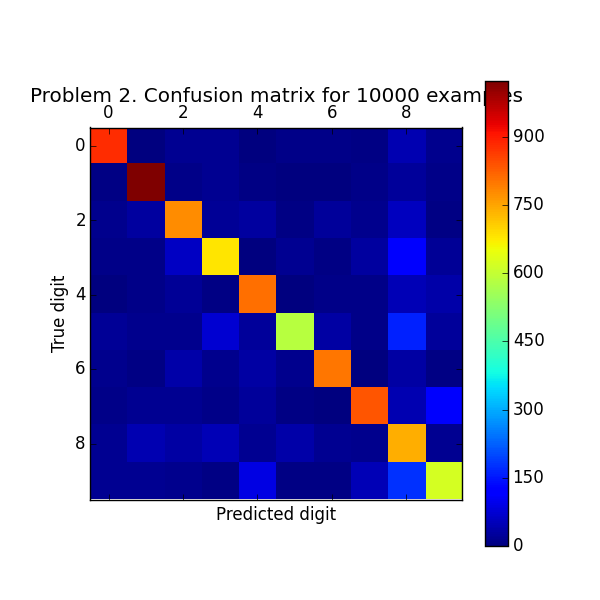
\includegraphics[scale=0.6]{figure8}

\newpage
\section*{Problem 3. solution}
One main reasons for using cross-validation instead of partition data as problem 1 and 2 is that the model does not fit the validation data as well as it fits the training data which is called overfitting. Thus, using cross-validation can avoid this and experiment the value C more accuracy.

The optimal parameter C that I found is 0.00000025.

Train an SVM with this value of C, the validation error rate is 0.14359999999999995

\section*{Problem 4. solution}
The optimal parameter C that I found is 40.

The accuracy using cross validation is 0.8062645011600927



\section*{Kaggle score:}

Highest score for Kaggle digits submission is 0.88020

Highest score for Kaggle spam submission is 0.76976


\newpage
\begin{lstlisting}
{digit_training.py}

import scipy.io as sio
from sklearn import svm
import random
import numpy as np
from sklearn.metrics import confusion_matrix
import matplotlib.pyplot as plt

if __name__ == '__main__':
	#read input
	trainData = sio.loadmat('./data/digit-dataset/train.mat')
	trainImages = trainData['train_images']

	#covert to array of 60,000's 28 x 28 arrays
	x_dim = len(trainImages)
	y_dim = len(trainImages[0])
	image_index = len(trainImages[0][0])
	trainImages = trainImages.transpose((2, 0, 1))
	trainImages = trainImages.reshape(image_index, x_dim * y_dim).tolist()

	actualLabels = np.transpose(trainData['train_labels'],(1, 0)).tolist()[0]

	#partition samples
	samples_indexs = [i for i in range(60000)]
	random.shuffle(samples_indexs)
	validation_sets_index = samples_indexs[:10000]
	validation_sets = []
	validation_sets_labels = []
	for index in validation_sets_index:
		validation_sets += [trainImages[index]]
		validation_sets_labels += [actualLabels[index]]
	samples_indexs = samples_indexs[10000:60000]

	error_rates = []
	#train classifler with 100 sample
	clf = svm.LinearSVC()
	print("Train 100 samples")
	random.shuffle(samples_indexs)
	small_samples_indexs = samples_indexs[:100]
	samples_sets = []
	samples_sets_labels = []
	for index in small_samples_indexs:
		samples_sets += [trainImages[index]]
		samples_sets_labels += [actualLabels[index]]

	clf.fit(samples_sets, samples_sets_labels)
	predict_labels = clf.predict(validation_sets)
	accuracy_indexs = [i for i in range(10000) if predict_labels[i] == validation_sets_labels[i]]
	accuracy = len(accuracy_indexs) / 10000
	print('The error rate is', 1 - accuracy)
	error_rates += [1 - accuracy]
	cm1 = confusion_matrix(validation_sets_labels, predict_labels)

	#train classifler with 200 sample
	clf = svm.LinearSVC()
	print("Train 200 samples")
	random.shuffle(samples_indexs)
	small_samples_indexs = samples_indexs[:200]
	samples_sets = []
	samples_sets_labels = []
	for index in small_samples_indexs:
		samples_sets += [trainImages[index]]
		samples_sets_labels += [actualLabels[index]]

	clf.fit(samples_sets, samples_sets_labels)
	predict_labels = clf.predict(validation_sets)
	accuracy_indexs = [i for i in range(10000) if predict_labels[i] == validation_sets_labels[i]]
	accuracy = len(accuracy_indexs) / 10000
	print('The error rate is', 1 - accuracy)
	error_rates += [1 - accuracy]
	cm2 = confusion_matrix(validation_sets_labels, predict_labels)

	#train classifler with 500 sample
	clf = svm.LinearSVC()
	print("Train 500 samples")
	random.shuffle(samples_indexs)
	small_samples_indexs = samples_indexs[:500]
	samples_sets = []
	samples_sets_labels = []
	for index in small_samples_indexs:
		samples_sets += [trainImages[index]]
		samples_sets_labels += [actualLabels[index]]

	clf.fit(samples_sets, samples_sets_labels)
	predict_labels = clf.predict(validation_sets)
	accuracy_indexs = [i for i in range(10000) if predict_labels[i] == validation_sets_labels[i]]
	accuracy = len(accuracy_indexs) / 10000
	print('The error rate is', 1 - accuracy)
	error_rates += [1 - accuracy]
	cm3 = confusion_matrix(validation_sets_labels, predict_labels)

	#train classifler with 1000 sample
	clf = svm.LinearSVC()
	print("Train 1000 samples")
	random.shuffle(samples_indexs)
	small_samples_indexs = samples_indexs[:1000]
	samples_sets = []
	samples_sets_labels = []
	for index in small_samples_indexs:
		samples_sets += [trainImages[index]]
		samples_sets_labels += [actualLabels[index]]

	clf.fit(samples_sets, samples_sets_labels)
	predict_labels = clf.predict(validation_sets)
	accuracy_indexs = [i for i in range(10000) if predict_labels[i] == validation_sets_labels[i]]
	accuracy = len(accuracy_indexs) / 10000
	print('The error rate is', 1 - accuracy)
	error_rates += [1 - accuracy]
	cm4 = confusion_matrix(validation_sets_labels, predict_labels)

	#train classifler with 2000 sample
	clf = svm.LinearSVC()
	print("Train 2000 samples")
	random.shuffle(samples_indexs)
	small_samples_indexs = samples_indexs[:2000]
	samples_sets = []
	samples_sets_labels = []
	for index in small_samples_indexs:
		samples_sets += [trainImages[index]]
		samples_sets_labels += [actualLabels[index]]

	clf.fit(samples_sets, samples_sets_labels)
	predict_labels = clf.predict(validation_sets)
	accuracy_indexs = [i for i in range(10000) if predict_labels[i] == validation_sets_labels[i]]
	accuracy = len(accuracy_indexs) / 10000
	print('The error rate is', 1 - accuracy)
	error_rates += [1 - accuracy]
	cm5 = confusion_matrix(validation_sets_labels, predict_labels)

	#train classifler with 5000 sample
	clf = svm.LinearSVC()
	print("Train 5000 samples")
	random.shuffle(samples_indexs)
	small_samples_indexs = samples_indexs[:5000]
	samples_sets = []
	samples_sets_labels = []
	for index in small_samples_indexs:
		samples_sets += [trainImages[index]]
		samples_sets_labels += [actualLabels[index]]

	clf.fit(samples_sets, samples_sets_labels)
	predict_labels = clf.predict(validation_sets)
	accuracy_indexs = [i for i in range(10000) if predict_labels[i] == validation_sets_labels[i]]
	accuracy = len(accuracy_indexs) / 10000
	print('The error rate is', 1 - accuracy)
	error_rates += [1 - accuracy]
	cm6 = confusion_matrix(validation_sets_labels, predict_labels)

	#train classifler with 10000 sample
	clf = svm.LinearSVC()
	print("Train 10000 samples")
	random.shuffle(samples_indexs)
	small_samples_indexs = samples_indexs[:10000]
	samples_sets = []
	samples_sets_labels = []
	for index in small_samples_indexs:
		samples_sets += [trainImages[index]]
		samples_sets_labels += [actualLabels[index]]

	clf.fit(samples_sets, samples_sets_labels)
	predict_labels = clf.predict(validation_sets)
	accuracy_indexs = [i for i in range(10000) if predict_labels[i] == validation_sets_labels[i]]
	accuracy = len(accuracy_indexs) / 10000
	print('The error rate is', 1 - accuracy)
	error_rates += [1 - accuracy]
	cm7 = confusion_matrix(validation_sets_labels, predict_labels)

	#plot graph for problem 1
	x_label = [100,200,500,1000,2000,5000,10000]
	plt.title('Problem 1. The error rates on validation set versus training example sizes')
	plt.xlabel('Traning sample size')
	plt.ylabel('Error rate')
	plt.plot(x_label, error_rates, 'bo-')
	plt.show()

	#plot confusion matrices for problem 2
	plt.matshow(cm1)
	plt.title('Problem 2. Confusion matrix for 100 examples')
	plt.colorbar()
	plt.ylabel('True digit')
	plt.xlabel('Predicted digit')
	plt.show()

	plt.matshow(cm2)
	plt.title('Problem 2. Confusion matrix for 200 examples')
	plt.colorbar()
	plt.ylabel('True digit')
	plt.xlabel('Predicted digit')
	plt.show()

	plt.matshow(cm3)
	plt.title('Problem 2. Confusion matrix for 500 examples')
	plt.colorbar()
	plt.ylabel('True digit')
	plt.xlabel('Predicted digit')
	plt.show()

	plt.matshow(cm4)
	plt.title('Problem 2. Confusion matrix for 1000 examples')
	plt.colorbar()
	plt.ylabel('True digit')
	plt.xlabel('Predicted digit')
	plt.show()

	plt.matshow(cm5)
	plt.title('Problem 2. Confusion matrix for 2000 examples')
	plt.colorbar()
	plt.ylabel('True digit')
	plt.xlabel('Predicted digit')
	plt.show()

	plt.matshow(cm6)
	plt.title('Problem 2. Confusion matrix for 5000 examples')
	plt.colorbar()
	plt.ylabel('True digit')
	plt.xlabel('Predicted digit')
	plt.show()

	plt.matshow(cm7)
	plt.title('Problem 2. Confusion matrix for 10000 examples')
	plt.colorbar()
	plt.ylabel('True digit')
	plt.xlabel('Predicted digit')
	plt.show()

	#problem 3. train 10000 samples with parameter C=0.00000025.
	#Use 10-fold cross validation training
	clf = svm.LinearSVC(C = 0.00000025)
	print("Train 10000 samples with parameter C = 0.00000025")
	random.shuffle(samples_indexs)
	small_samples_indexs = samples_indexs[:10000]
	samples_sets = []
	samples_sets_labels = []
	for index in small_samples_indexs:
		samples_sets += [trainImages[index]]
		samples_sets_labels += [actualLabels[index]]

	clf.fit(samples_sets, samples_sets_labels)
	predict_labels = clf.predict(validation_sets)
	accuracy_indexs = [i for i in range(10000) if predict_labels[i] == validation_sets_labels[i]]
	accuracy = len(accuracy_indexs) / 10000
	print('The error rate is', 1 - accuracy)

\end{lstlisting}


\newpage
\begin{lstlisting}
{find_parameter_C_for_digit.py}

import scipy.io as sio
from sklearn import svm
import random
import numpy as np

if __name__ == '__main__':
	#read input
	trainData = sio.loadmat('./data/digit-dataset/train.mat')
	trainImages = trainData['train_images']

	#covert to array of 60,000's 28 x 28 arrays
	x_dim = len(trainImages)
	y_dim = len(trainImages[0])
	image_index = len(trainImages[0][0])
	trainImages = trainImages.transpose((2, 0, 1))
	trainImages = trainImages.reshape(image_index, x_dim * y_dim).tolist()

	actualLabels = np.transpose(trainData['train_labels'],(1, 0)).tolist()[0]

	#chose random 10000 image as training samples
	samples_indexs = [i for i in range(60000)]
	random.shuffle(samples_indexs)
	sample_sets_index = samples_indexs[:10000]
	sample_sets = []
	sample_sets_labels = []
	for index in sample_sets_index:
		sample_sets += [trainImages[index]]
		sample_sets_labels += [actualLabels[index]]

	sample_sets = np.reshape(sample_sets, (10, 1000, x_dim * y_dim)).tolist()
	sample_sets_labels = np.reshape(sample_sets_labels, (10, 1000)).tolist()

	#start 10-fold cross validation training
	accuracies = 0
	clf = svm.LinearSVC(C = 0.00000025)
	print("10-fold cross-validation training on 10000 samples")
	print("C = 0.00000025", )
	for i in range(10):
		print("iteration", i)
		for j in range(10):
			if j != i:
				clf.fit(sample_sets[j], sample_sets_labels[j])
		predict_labels = clf.predict(sample_sets[i])
		accuracy_indexs = [j for j in range(1000) if predict_labels[j] == sample_sets_labels[i][j]]
		accuracy = len(accuracy_indexs) / 1000
		accuracies += accuracy
	average_accuracy = accuracies / 10
	print('The accuracy rate is', average_accuracy)



\end{lstlisting}


\newpage
\begin{lstlisting}
{find_parameter_C_for_spam.py}
import scipy.io as sio
from sklearn import svm
import random
import numpy as np

if __name__ == '__main__':
	#read input
	trainData = sio.loadmat('./data/spam-dataset/spam_data.mat')
	trainImages = trainData['training_data'].tolist()
	actualLabels = trainData['training_labels'].tolist()[0]

	#chose random 5172 data as training samples
	samples_indexs = [i for i in range(5172)]
	random.shuffle(samples_indexs)
	sample_sets_index = samples_indexs[:5172]
	sample_sets = []
	sample_sets_labels = []
	for index in sample_sets_index:
		sample_sets += [trainImages[index]]
		sample_sets_labels += [actualLabels[index]]

	sample_sets = np.reshape(sample_sets, (6, 862, 32)).tolist()
	sample_sets_labels = np.reshape(sample_sets_labels, (6, 862)).tolist()

	#start 6-fold cross validation training
	accuracies = 0
	clf = svm.LinearSVC(C = 40)
	print("6-fold cross-validation training on 5172 samples")
	print("C = 40", )
	for i in range(6):
		print("iteration", i)
		for j in range(6):
			if j != i:
				clf.fit(sample_sets[j], sample_sets_labels[j])
		predict_labels = clf.predict(sample_sets[i])
		accuracy_indexs = [j for j in range(862) if predict_labels[j] == sample_sets_labels[i][j]]
		accuracy = len(accuracy_indexs) / 862
		accuracies += accuracy
	average_accuracy = accuracies / 6
	print('The accuracy rate is', average_accuracy)


\end{lstlisting}


\newpage
\begin{lstlisting}
{kaggle_digit_submission.py}
import scipy.io as sio
from sklearn import svm
import random
import numpy as np
import csv


#Use to write CSV format file for kaggle_digit submisiion with required SVM model
if __name__ == '__main__':
	#train SVM model
	trainData = sio.loadmat('./data/digit-dataset/train.mat')
	trainImages = trainData['train_images']

	x_dim = len(trainImages)
	y_dim = len(trainImages[0])
	image_index = len(trainImages[0][0])
	trainImages = trainImages.transpose((2, 0, 1))
	trainImages = trainImages.reshape(image_index, x_dim * y_dim).tolist()

	actualLabels = np.transpose(trainData['train_labels'],(1, 0)).tolist()[0]

	samples_indexs = [i for i in range(60000)]
	random.shuffle(samples_indexs)
	random.shuffle(samples_indexs)
	sample_sets_index = samples_indexs[:60000]
	sample_sets = []
	sample_sets_labels = []
	for index in sample_sets_index:
		sample_sets += [trainImages[index]]
		sample_sets_labels += [actualLabels[index]]

	#training with optimal value C
	clf = svm.LinearSVC(C = 0.0000001)
	clf.fit(sample_sets, sample_sets_labels)

	#predit result
	testData = sio.loadmat('./data/digit-dataset/test.mat')
	testImages = testData['test_images']
	x_dim = len(testImages)
	y_dim = len(testImages[0])
	image_index = len(testImages[0][0])
	testImages = testImages.transpose((2, 0, 1))
	testImages = testImages.reshape(image_index, x_dim * y_dim).tolist()

	predict_labels = clf.predict(testImages)
	indexs = [i for i in range(1, 10001)]
	data = []
	data += [indexs]
	data += [predict_labels]
	data = np.transpose(data, (1, 0)).tolist()
	first_row = [['Id', 'Category']]
	with open('digitpredict.csv', 'w') as f:
	    a = csv.writer(f)
	    a.writerows(first_row)
	    a.writerows(data)




\end{lstlisting}


\newpage
\begin{lstlisting}
{kaggle_spam_submission.py.py}

import scipy.io as sio
from sklearn import svm
import random
import numpy as np
import csv


#Use to write CSV format file for kaggle_digit submisiion with required SVM model
if __name__ == '__main__':
	#train SVM model
	trainData = sio.loadmat('./data/spam-dataset/spam_data.mat')
	trainImages = trainData['training_data'].tolist()
	actualLabels = trainData['training_labels'].tolist()[0]

	#chose random 10000 image as training samples
	samples_indexs = [i for i in range(5172)]
	random.shuffle(samples_indexs)
	sample_sets_index = samples_indexs[:5172]
	sample_sets = []
	sample_sets_labels = []
	for index in sample_sets_index:
		sample_sets += [trainImages[index]]
		sample_sets_labels += [actualLabels[index]]

	clf = svm.LinearSVC(C = 40)
	clf.fit(sample_sets, sample_sets_labels)

	#predit result
	testImages = trainData['test_data']

	predict_labels = clf.predict(testImages)
	indexs = [i for i in range(1, 5858)]
	data = []
	data += [indexs]
	data += [predict_labels]
	data = np.transpose(data, (1, 0)).tolist()
	first_row = [['Id', 'Category']]
	with open('spampredict.csv', 'w') as f:
	    a = csv.writer(f)
	    a.writerows(first_row)
	    a.writerows(data)





\end{lstlisting}

\end{document}